\documentclass[Ligatures=TeX,table,brazil,svgnames,usetotalslideindicator,comp
ress,10pt]{beamer}

\usetheme[titleformat=allsmallcaps]{metropolis}

\usepackage{polyglossia}
\setdefaultlanguage{brazil}
\disablehyphenation

\usepackage[cachedir=/tmp/minted-\jobname]{minted}
\usemintedstyle{pastie}

\usepackage{graphicx}
\graphicspath{{./figuras/}}

%\usepackage{textpos}

%\usepackage{xspace}
%\usepackage{mdwlist}
%\usepackage{siunitx}
\usepackage{alltt}
\usepackage{multicol}
\usepackage{multirow}
%\usepackage{amsmath}

\usepackage{cancel}
%\usepackage[simplified]{pgf-umlcd}
%\usepackage{pgf-umlsd}

\usepackage{smartdiagram}

\newcommand{\setcoverbg}{
    \setbeamertemplate{background}
     {
\includegraphics[width=\paperwidth,height=\paperheight]{backgrounds/coverbg}}
}
\newcommand{\setintersectionbg}{
    \setbeamertemplate{background}
     {
\includegraphics[width=\paperwidth,height=\paperheight]{backgrounds/blank}}
}
\newcommand{\setsectionbg}{
    \setbeamertemplate{background}
     {
\includegraphics[width=\paperwidth,height=\paperheight]{backgrounds/slidebg2}}
}


\title{Introdução}

\subtitle{MCTA025-13 - Sistemas Distribuídos}

\author{Emilio Francesquini\\e.francesquini@ufabc.edu.br}
\institute{Centro de Matemática, Computação e Cognição\\ Universidade Federal do ABC}
\date{04 de junho de 2018}

\begin{document}

\setcoverbg
\maketitle

\setsectionbg

\begin{frame}
  \frametitle{Informações de contato}
  \begin{itemize}
  \item Prof. Dr. Emilio Francesquini
  \item \url{e.francesquini@ufabc.edu.br}
  \item \url{http://professor.ufabc.edu.br/~e.francesquini}
  \item Santo André, Bloco A, Sala 531-2
  \end{itemize}
\end{frame}

\setintersectionbg
\begin{frame}[standout]
  Todas as informações relativas à disciplina tais como:
  \begin{itemize}
      \item Datas importantes
      \item Critérios de avaliação
      \item Bibliografia
      \item Avisos
      \item \ldots
  \end{itemize}
  Estarão disponíveis em:
  \normalsize{\url{http://professor.ufabc.edu.br/~e.francesquini/sd/}}
\end{frame}
\setsectionbg

\begin{frame}
  \frametitle{Disclaimer}
  \begin{itemize}
  \item Estes slides foram preparados para o curso de \textbf{Sistemas
      Distribuídos na UFABC}.
  \item Este material pode ser usado livremente desde que sejam
    mantidos, além deste aviso, os créditos aos autores e
    instituições.
  \item Estes slides foram adaptados daqueles originalmente preparados
    (e gentilmente cedidos) pelo professor \textbf{Daniel Cordeiro, da
      EACH-USP} que por sua vez foram baseados naqueles
    disponibilizados online pelos autores do livro ``Distributed
    Systems'', 3ª Edição em:
    \url{https://www.distributed-systems.net}.

  \end{itemize}
\end{frame}


\begin{frame}
  \frametitle{Informações gerais}

  \begin{block}{Multitasking}
    \begin{quotation}
      Attention, multitaskers (if you can pay attention, that is):
      Your brain may be in trouble.

      People who are regularly bombarded with several streams of
      electronic information do not pay attention, control their
      memory or switch from one job to another as well as those who
      prefer to complete one task at a time, a group of Stanford
      researchers has found.

      (...)

      So maybe it’s time to stop e-mailing if you’re following the
      game on TV, and rethink singing along with the radio if you’re
      reading the latest news online. By doing less, you might
      accomplish more.
    \end{quotation}
  \end{block}

  \begin{flushright}
    \tiny
    \url{http://news.stanford.edu/2009/08/24/multitask-research-study-082409/}
  \end{flushright}

\end{frame}

\begin{frame}
  \frametitle{O perigo de fazer várias coisas ao mesmo tempo}
  \begin{itemize}
  \item Veja o vídeo de Clifford Nass (Stanford) em \url{https://youtu.be/PriSFBu5CLs}
  \item Se render às distrações do mundo digital (e-mail, mensagens
    instantâneas, Facebook, etc.) faz o cérebro lançar pequenas doses
    de dopamina
  \item Com o tempo, ficamos viciados nisso
  \item Resultado: \textit{multitaskers} gastam muito mais poder de processamento cerebral do que \textit{monotaskers} quando são destraídos
  \item Efeitos a longo prazo são difíceis de reverter
  \end{itemize}
\end{frame}

\begin{frame}
  \frametitle{Por isso, na sala de aula:}

  \begin{onlyenv}<1>
    \begin{figure}
      \centering
      
\includegraphics[width=.3\textwidth]{no-phone}
      \begin{flushright}
        \tiny
        No Phone by Rflor from the Noun Project
      \end{flushright}
    \end{figure}
  \end{onlyenv}

  \begin{onlyenv}<2>
    \begin{figure}
      \centering
      
\includegraphics[width=.5\textwidth]{no-laptop}
      \begin{flushright}
        \tiny
        blocked laptop by unlimicon from the Noun Project
      \end{flushright}
    \end{figure}
  \end{onlyenv}

    \begin{onlyenv}<3>
    \begin{figure}
      \centering
      
\includegraphics[width=.7\textwidth]{social-media}
    \end{figure}
  \end{onlyenv}
\end{frame}

\begin{frame}
  \frametitle{Alunos com Deficiência}

  Avise seu professor \textbf{o quanto antes} sobre a necessidade de cuidados extras para acessibilidade nos casos de deficiência:
  \begin{itemize}
  \item visual,
  \item física,
  \item auditiva,
  \item dislexia,
  \item etc.
  \end{itemize}

  \url{http://proap.ufabc.edu.br/}

\end{frame}

\begin{frame}
  \frametitle{Aulas teóricas}

  \begin{itemize}
  \item Professor: Emilio Francesquini --- \url{e.francesquini@ufabc.edu.br}
  \item Aulas:
    \begin{itemize}
    \item Segunda das 21:00 às 23:00, semanal, Sala A-107-0
    \item Quarta das 19:00 às 21:00, quinzenal I, Sala A-108-0
    \end{itemize}
  \end{itemize}
\end{frame}

\begin{frame}
  \frametitle{Aulas Práticas}
  Quartas, das 19:00 às 21:00, quinzenal II

  \begin{itemize}
  \item Turma NA1 --- NA1MCTA025-13SA
    \begin{itemize}
    \item Professor: Emilio Francesquini
    \item Sala: 409-2
    \end{itemize}
  \item Turma NA2 --- NA2MCTA025-13SA
    \begin{itemize}
    \item Professor: Fernando Teubl Ferreira
    \item Sala: 407-2
    \end{itemize}
  \end{itemize}
\end{frame}

\begin{frame}
  \frametitle{Atendimento}
  \begin{itemize}
  \item Teoria e Prática (Turma NA1) - Prof. Emilio Francesquini
    \begin{itemize}
    \item Presencial
      \begin{itemize}
      \item Na própria sala de aula, após as aulas.
      \item Quarta-feira, das 17:00 às 19:00, sala 531-2.
      \item Agendado por e-mail.
      \end{itemize}
    \item Online
      \begin{itemize}
      \item Por e-mail.
      \item Pelo fórum da disciplina (TIDIA --- Procure por \\``SD - 2018.Q2 - Teoria - Turmas NA1 e NA2'')
      \end{itemize}
    \end{itemize}
  \item Prática (Turma NA2) --- Prof. Fernando Teubl Ferreira
    \begin{itemize}
    \item Quarta-feira, das 17:00 às 19:00, sala 525-2.
    \end{itemize}
  \end{itemize}
\end{frame}

\begin{frame}
  \frametitle{Honestidade Acadêmica}

\begin{columns}
  \column{0.25\linewidth}
  \centering
  
\includegraphics[width=3cm]{palm.pdf}
  \column{0.7\linewidth}
  Qualquer tentativa de fraude nas provas, listas de exercícios ou projetos implicará:
  \begin{itemize}
  \item\textbf{Conceito final CF = F (reprovado)} para \textbf{TODOS} os envolvidos.
  \item \textbf{Denúncia apresentada à Comissão de Transgressões Disciplinares
    Discentes da Graduação}, a qual decidirá sobre a punição adequada à
    violação que pode resultar em \textbf{advertência, suspensão ou
    desligamento}, de acordo com os artigos 78-82 do Regimento Geral da
    UFABC.
  \item \textbf{Denúncia apresentada à Comissão de Ética da UFABC}, de acordo
    com o artigo 25 do Código de Ética da UFABC.
  \end{itemize}
\end{columns}
\end{frame}

\begin{frame}
  \frametitle{Critérios de Avaliação}
  A avaliação da disciplina será composta por duas notas, uma referente
à teoria e outra à prática. Considere:

\begin{itemize}
\item \(N_F\) é a nota final;
\item \(N_T\) é a nota de teoria;
\item \(N_P\) é a nota de prática.
\end{itemize}


A nota final \(N_F\) será determinada da seguinte maneira:

\begin{equation*}
N_F =
    \begin{cases}
        \min\{N_T, N_P\}                ,& \text{se } N_T < 5 \text{ ou } N_P < 5 \\
        0.6 \cdot N_T + 0.4 \cdot N_P ,& \text{caso contrário}
    \end{cases}
\end{equation*}

\end{frame}

\begin{frame}
  \frametitle{Critérios de Avaliação - Conceito Final}
  O conceito final \(C_F\) será obtido de acordo com a equação abaixo:

\begin{equation*}
C_F =
    \begin{cases}
    \textbf{O} ,& \text{se ausência total exceder 25\%}\\
    \textbf{F} ,& \text{se } N_F \in [0,0;5,0) \\
    \textbf{D} ,& \text{se } N_F \in [5,0;6,0) \\
    \textbf{C} ,& \text{se } N_F \in [6,0;7,0) \\
    \textbf{B} ,& \text{se } N_F \in [7,0;8,5) \\
    \textbf{A} ,& \text{se } N_F \in [8,5;10,0] \\
    \end{cases}
\end{equation*}
\end{frame}

\begin{frame}
  \frametitle{Avaliação de Teoria}
  A nota de teoria \(N_T\) será formada por duas provas \(P_1\) e \(P_2\),
  de pesos iguais.  Todas as provas serão efetuadas em sala de aula,
  sem auxílio de computador.



  Haverá também uma prova subsitutiva \(P_S\) que será aberta a todos
  os interessados, ainda que eles tenham feito tanto a \(P_1\) quanto
  a \(P_2\).

  \textbf{ATENÇÃO} --- A nota da PS será utilizada obrigatoriamente em
  substituição à menor nota entre \(P_1\) e \(P_2\) ainda que isto
  diminua a nota final do aluno!
\begin{equation*}
N_T =
    \begin{cases}
    \frac {\max \{P_1, P_2\} + P_S}{2} ,& \text{caso tenha feito a } P_S \\
    \frac {P_1 + P_2}{2}               ,& \text{caso contrário}
    \end{cases}
\end{equation*}

\end{frame}


\begin{frame}
  \frametitle{Avaliação de Prática}

  A avaliação da prática será feita através de dois projetos
  \(\text{Pr}_1\) e \(\text{Pr}_2\) de igual peso. Sua nota será,
  então, calculada pela seguinte equação:

\begin{equation*}
N_P = \frac {\text{Pr}_1 + \text{Pr}_2}{2}
\end{equation*}

\end{frame}


\begin{frame}
  \frametitle{Recuperação} A Resolução ConsEPE nº 182 garante a todos
  os alunos com \(C_F\) igual a \textbf{D} ou \textbf{F} o direito a
  fazer uso de mecanismos de recuperação.

A recuperação será feita através de uma prova \(P_R\), sem consulta,
e a sua nota será utilizada para compor a o conceito
pós-recuperação \(C_R\) conforme as equações abaixo:

$$N_R = \frac{P_R + N_F}{2}$$

\textbf{Caso 1 \(C_F = D\):}

\begin{equation*}
C_R =
    \begin{cases}
    \textbf{C} ,& \text{se } N_R \geq 6,0 \\
    \textbf{D} ,& \text{caso contrário}
    \end{cases}
\end{equation*}

\textbf{Caso 2 \(C_F = F\):}
\begin{equation*}
C_R =
    \begin{cases}
    \textbf{D} ,& \text{se } N_R \geq 5,0 \\
    \textbf{F} ,& \text{caso contrário}
    \end{cases}
\end{equation*}
\end{frame}


\begin{frame}
  \frametitle{Datas Importantes}
  \begin{itemize}
  \item \textbf{Prova 1} --- 16/07/2018
  \item \textbf{Prova 2} --- 27/08/2018
  \item \textbf{Prova Substitutiva} --- 28/08/2018
  \item \textbf{Prova de Recuperação} --- 17/09/2018 --- Horário a definir
  \item \textbf{Projeto 1} --- A definir
  \item \textbf{Projeto 2} --- A definir
  \end{itemize}
\end{frame}

\begin{frame}
  \frametitle{Livro texto}
  \begin{itemize}
  \item \textbf{[ST] --- Distributed Systems 3rd edition} (2017), por Maarten van Steen e Andrew S. Tanenbaum
  \item \url{https://www.distributed-systems.net/index.php/books/distributed-systems-3rd-edition-2017/}
  \item Tópicos:
    \begin{itemize}
    \item Introdução;
    \item Arquiteturas de sistemas distribuídos;
    \item Processos;
    \item Comunicação;
    \item Nomes;
    \item MapReduce;
    \item Coordenação;
    \item Modelos de Consistência;
    \end{itemize}
  \end{itemize}

\end{frame}

\begin{frame}
  \frametitle{Bibliografia adicional}
  \begin{itemize}
  \item  \textbf{[CDKB]} Coulouris, J. Dollimore, T. Kindberg, and
    G. Blair. \textbf{Distributed Systems: Concepts and Design}. 5th Edition,
    Addison-Wesley, 2011.
  \item \textbf{[KS]} A.D. Kshemkalyani, M. Singhal, \textbf{Distributed Computing:
      Principles, Algorithms, and Systems}. Paperback edition, Cambridge
    University Press, 2011.
  \item \textbf{[NL]} Lynch, Nancy Ann. \textbf{Distributed algorithms}, Morgan Kaufmann
    Publishers, 1997.
  \end{itemize}

  Versões disponíveis na biblioteca tanto em português quanto em
  inglês. Contudo, (em particular as versões em português) podem ser
  de edições anteriores. Veja página da disciplina para mais detalhes.
\end{frame}


\setintersectionbg
\begin{frame}[standout]
  O que é um Sistema Distribuído?
\end{frame}

\setsectionbg
\begin{frame}
  \frametitle{Todos já devem ter ouvido algo sobre Cloud Computing}

  Ou ao menos algumas dessas ideias:

  \setbeamercovered{transparent}
  \begin{itemize}[<+->]
  \item ``Computação em nuvem finalmente tornou realidade o sonho da
    computação utilitária''
  \item ``Desenvolvedores não precisam mais se preocupar em conseguir
    grandes somas de dinheiro antes de colocar uma nova aplicação web
    no ar''
  \item ``Adeus aos problemas de provisionamento de servidores
    (Elasticidade dos recursos)''
  \item Software como um serviço
  \item Plataforma como um serviço
  \item Infraestrutura como um serviço
  \end{itemize}

\end{frame}

\begin{frame}
  \frametitle{Quatro problemas que (ainda) requerem\\ constante inovação
    tecnológica}

  \begin{itemize}
  \item Problemas ``em escala da web''
  \item \textbf{Grandes} \textit{data centers}
  \item Computação paralela e distribuída
  \item Aplicações web interativas
  \end{itemize}

\end{frame}

\begin{frame}
  \frametitle{Problemas em escala da web}

  \begin{itemize}
  \item Características
    \begin{itemize}
    \item Definitivamente \textit{data-intensive}
    \item Mas podem também ser \textit{processing-intensive}
    \end{itemize}
  \item Exemplos:
    \begin{itemize}
    \item \textit{Crawling}, indexação, busca, mineração de dados da
      web
    \item Pesquisa em biologia computacional na era ``pós-genômica''
    \item Processamento de dados científicos (física, astronomia, etc.)
    \item Redes de sensores
    \item Aplicações Web 2.0
    \item etc.
    \end{itemize}
  \end{itemize}

\end{frame}

\begin{frame}
  \frametitle{De qual volume de dados estamos falando?}

  \only<1> {
    \begin{block}{}
      Problemas da ordem de \alert{petabytes}!
    \end{block}
    \begin{align*}
      1 \text{ PB} &= 1.000.000.000.000.000 \text{ B}\\
           &= 1.000^5 \text{ B}\\
           &= 10^{15} \text{ B}\\
           &= 1 \text{ milhão de gigabytes}\\
           &= 1 \text{ mil terabytes}
    \end{align*}
  }

  \only<2-6> {
  \begin{block}{Muitos, mas \textbf{muitos} dados}
    \setbeamercovered{transparent}
    \begin{itemize}
    \item<2-> O Google processa cerca de \textbf{20 petabytes} de dados
      por dia (2008)
    \item<3-> O Wayback Machine tem cerca de \textbf{3 petabytes + 100
        terabytes/dia} (mar/2009)
    \item<4-> O Facebook tem cerca de \textbf{2,5 petabytes de dados de
        usuários + 15 terabytes/dia} (abr/2009)
    \item<5-> O site eBay tem cerca de \textbf{6,5 petabytes de dados dos usuários + 50 terabytes/dia} (mai/2009)
    \item<6-> O Grande Colisor de Hádrons do CERN irá gerar cerca de \textbf{15 petabytes/ano}
    \end{itemize}
  \end{block}
  }

  \only<7> {
    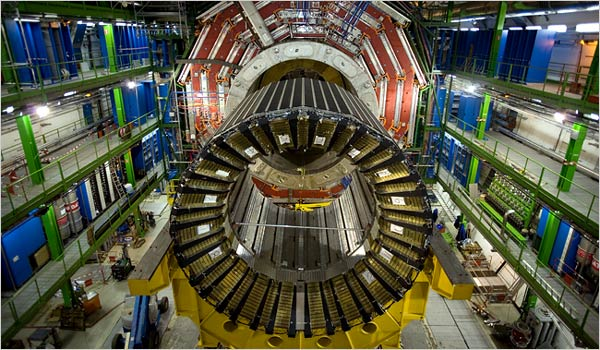
\includegraphics[width=\linewidth]{cern}
  }

  \only<8> {
    \begin{align*}
      1 \text{ PB} &= 1.000.000.000.000.000 \text{ B}\\
           &= 1.000^5 \text{ B}\\
           &= 10^{15} \text{ B}\\
           &= 1 \text{ milhão de gigabytes}\\
           &= 1 \text{ mil terabytes}
    \end{align*}

  \begin{block}{}
    Ou seja, os \alert{15 petabytes} que o CERN irá gerar por ano equivalem a \alert{15
    milhões de gigabytes}. Seriam necessários \alert{1,7 milhão de DVDs
    \textit{dual-layer}} para armazenar tanta informação!
  \end{block}
  }

\end{frame}

\begin{frame}
  \frametitle{O que se faz com tantos dados?}

  \setbeamercovered{transparent}
  \begin{itemize}
  \item Encontram informações sobre novos fatos
    \begin{itemize}
    \item Casamento de padrões com informações da web
    \item ex: quem matou John Lennon?
    \end{itemize}
  \item<2-> Procuram por novas relações entre os dados
    \begin{itemize}
    \item<2-> Alguns padrões levam a novas relações:
      \begin{itemize}
      \item<3-> os fatos: ``Nascimento-de(Mozart, 1756)'' e ``Nascimento-de(Einstein, 1879)''
      \item<4-> levam aos dados: ``Wolfgang Amadeus Mozart
        (1756--1791)'' e ``Einstein nasceu em 1879''
      \item<5-> que levam a diferentes padrões: ``PESSOA (DATA --'' e ``PESSOA nasceu em DATA''
      \item<6-> que, por sua vez, permitem encontrar novos fatos
      \end{itemize}
    \end{itemize}
  \end{itemize}

\end{frame}

\begin{frame}
  \frametitle{Como resolver problemas tão grandes?}

  Estratégia simples (mas de difícil execução):

  \begin{itemize}
  \item Dividir para conquistar
  \item Usar mais recursos computacionais a medida que mais dados aparecerem
  \end{itemize}

\end{frame}

\begin{frame}
  \frametitle{Grandes data centers}

  \begin{block}{Pergunta:}
    Quão grandes são os \textit{data centers} que fazem sistemas que
    afetam a vida de quase todo mundo que se conecta a Internet (como
    os do Google, Facebook, etc.) funcionarem?
  \end{block}

\end{frame}

\begin{frame}
  \frametitle{Grandes data centers}

  \begin{center}
    \includegraphics<1>[width=.9\linewidth]{google1}
    \includegraphics<2>[width=.9\linewidth]{google2}
    \includegraphics<3>[width=.9\linewidth]{google3}
    \includegraphics<4>[width=.9\linewidth]{google4}
  \end{center}

  \begin{flushright}
  \tiny
  Fonte: \url{http://www.google.com/intl/pt-BR/about/datacenters/}
  \end{flushright}

\end{frame}

\begin{frame}
  \frametitle{Grandes data centers}

  \begin{block}{}
      Só o Google tem \alert{treze} desses espalhados pelo mundo!
  \end{block}

\begin{overlayarea}{\linewidth}{5cm}
  \only<1>{
  \begin{block}{Américas}
    \begin{itemize}
    \item Berkeley County, Carolina do Sul
    \item Council Bluffs, Iowa
    \item Douglas County, Georgia
    \item Mayes County, Oklahoma
    \item Lenoir, Carolina do Norte
    \item The Dalles, Oregon
    \item Quilicura, Chile
   \end{itemize}
  \end{block}}

\only<2>{
  \begin{block}{Ásia}
\begin{itemize}
\item    Hong Kong
   \item Cingapura
   \item Taiwan
   \end{itemize}
 \end{block}}

\only<3>{
\begin{block}{Europa}
\begin{itemize}
\item    Hamina, Finlândia
    \item St Ghislain, Bélgica
    \item Dublin, Irlanda
    \end{itemize}
  \end{block}}
\end{overlayarea}

\end{frame}


\begin{frame}
  \Huge Como isso era feito até então?
\end{frame}

\begin{frame}
  \frametitle{Evolução da computação}
    \setbeamercovered{transparent}
    \begin{itemize}[<+->]
    \item anos 50: computadores eram grandes calculadoras programadas
      com cartões perfurados; início da computação paralela
    \item final dos anos 60: ARPANET (computadores começavam a serem
      interconectados; noção de computação \emph{como um serviço})
    \item anos 70: surgem os primeiros microprocessadores
    \item anos 80: popularização dos computadores pessoais
    \item anos 90: popularização da Internet
    \end{itemize}
\end{frame}

\begin{frame}
  \frametitle{Paradigmas de computação}

  \setbeamercovered{transparent}
  \begin{itemize}[<+->]
  \item Computadores Pessoais
  \item Computadores Paralelos
  \item Aglomerados de Computadores (\textit{clusters})
  \item Computação Voluntária (\textit{Volunteer Computing}):
    \begin{itemize}
    \item The Great Internet Mersenne Prime Search (1996): busca por
      primos de Mersenne (primos da forma $2^n-1, n \in \mathbb{N}$)
    \item distributed.net (1997): decriptografia por força-bruta
    \item SETI@Home (1999): análise de sinais de rádio vindos do
      espaço em busca de evidência de vida extra-terreste
    \end{itemize}
  \item Computação em Grade (\textit{Grid Computing})
  \end{itemize}
\end{frame}

\section{Problemas atuais}

\begin{frame}
  \Huge E como é feito agora?
\end{frame}

\begin{frame}
  \frametitle{Grandes data centers}

  \setbeamercovered{transparent}
  \begin{itemize}[<+->]
  \item Seu problema aumenta na mesma escala da web?\\\textbf{Fácil:} basta adicionar mais máquinas
  \item Tendência: centralização dos recursos computacionais em
    grandes data centers
    \begin{itemize}
    \item O que os \emph{fiordes noruegueses}, a \emph{Islândia}, o estado americano
      do \emph{Oregon} e \emph{minas abandonadas} tem em comum?
    \end{itemize}
  \item Problemas a serem resolvidos:
    \begin{itemize}
    \item Redundância
    \item Eficiência
    \item Utilização
    \item Gerenciamento
    \end{itemize}
  \end{itemize}

\end{frame}

\begin{frame}
  \frametitle{Ideias principais}

  \begin{itemize}
  \item Escalabilidade horizontal, não vertical
    \begin{itemize}
    \item Existem limites para máquinas SMP e arquiteturas de memória compartilhada
    \end{itemize}
  \item Mova o processamento para perto dos dados
    \begin{itemize}
    \item a banda de rede é limitada
    \end{itemize}
  \item Processe os dados sequencialmente, evite padrões de acesso
    aleatórios
    \begin{itemize}
    \item \textit{seeks} são custosos, mas a vazão
      (\textit{throughput}) do disco é razoável
    \end{itemize}
  \end{itemize}

\end{frame}

\begin{frame}
  \frametitle{Como programar aplicações escaláveis?}

  Divisão e conquista

  \begin{figure}
    \centering
    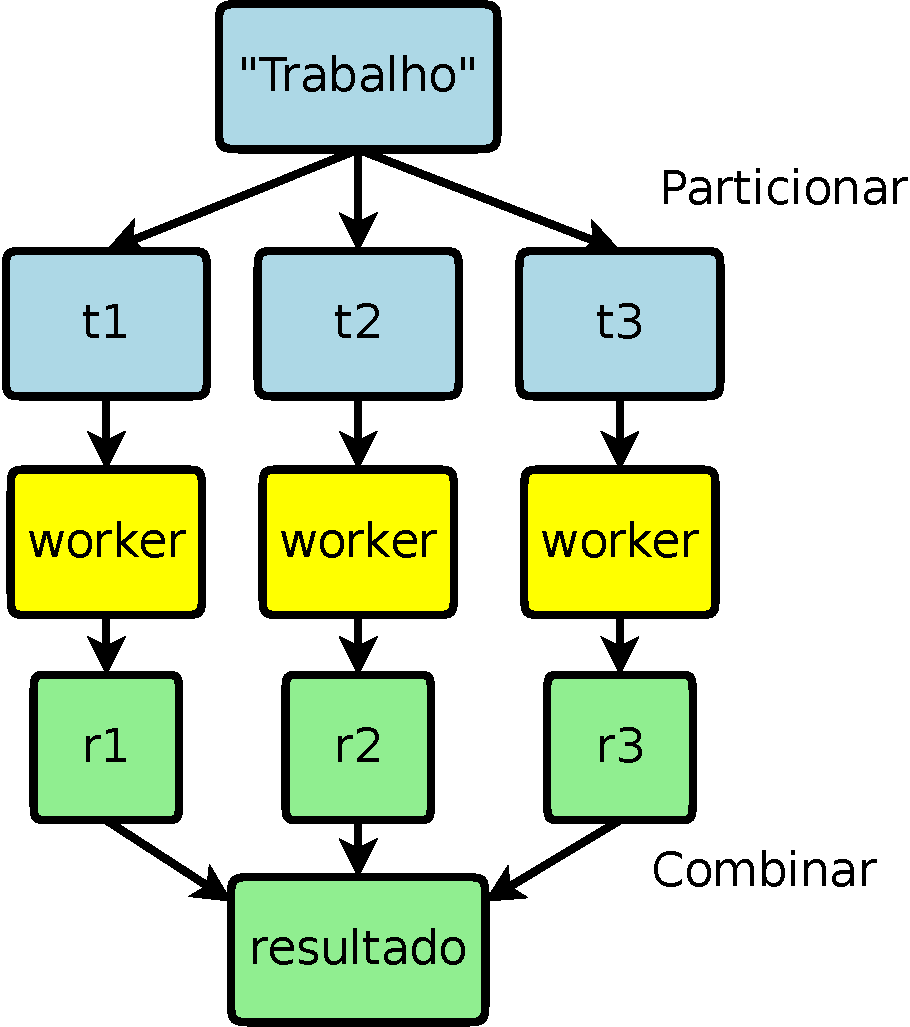
\includegraphics[scale=0.35]{divisao-conquista}
  \end{figure}

\end{frame}

\begin{frame}
  \frametitle{Desafios de paralelização}
  \begin{itemize}
  \item Como repartir as unidades de trabalho entre os \textit{workers}?
  \item O que fazer quando temos mais trabalho do que \textit{workers}?
  \item E se os \textit{workers} precisarem compartilhar resultados
    intermediários entre si?
  \item Como agregar os resultados parciais?
  \item O que fazer se um \textit{worker} parar de funcionar?
  \item Como saber se todos os \textit{workers} terminaram seus trabalhos?
  \end{itemize}
\end{frame}

\begin{frame}
  \frametitle{Problema recorrente}

  \begin{itemize}
  \item Problemas de paralelização surgem por causa de:
    \begin{itemize}
    \item comunicação entre os \textit{workers}
    \item acesso a recursos compartilhados (por exemplo, dados)
    \end{itemize}
  \item Portanto, precisamos de algum mecanismo de sincronização
  \end{itemize}

\end{frame}

\begin{frame}
  \frametitle{Gerenciar múltiplos workers}

  \begin{itemize}
  \item É difícil, pois:
    \begin{itemize}
    \item Não sabemos em que ordem cada \textit{worker} será executado
    \item Não sabemos quando um \textit{worker} irá interromper outro \textit{worker}
    \item Não sabemos em qual ordem os \textit{workers} irão acessar
      os dados compartilhados
    \end{itemize}
  \item Por tanto, nós precisamos de:
    \begin{itemize}
    \item Semáforos (\texttt{lock}, \texttt{unlock})
    \item Variáveis condicionais (\texttt{wait}, \texttt{notify}, \texttt{broadcast})
    \item Barreiras de sincronização
    \end{itemize}
  \item Ainda assim, restam problemas como:
    \begin{itemize}
    \item Deadlock, starvation, race coditions, ...
    \end{itemize}
  \end{itemize}

\end{frame}

\begin{frame}
  \frametitle{Ferramentas atuais}
  \begin{itemize}
  \item Modelos de programação:
    \begin{itemize}
    \item Memória compartilhada (pthreads)
    \item Passagem de mensagens (MPI)
    \end{itemize}
  \item Padrões arquiteturais:
    \begin{itemize}
    \item Mestre--escravo
    \item Produtor--consumidor
    \item Filas de trabalho compartilhadas
    \end{itemize}
  \end{itemize}
\end{frame}

\begin{frame}
  \frametitle{Moral da história}
  \begin{itemize}
  \item Tudo se resume ao nível mais adequado de abstração
  \item Esconda os detalhes do sistema dos desenvolvedores
    \begin{itemize}
    \item Evita os problemas com race conditions, contenção em locks, etc.
    \end{itemize}
  \item Separe o \alert{``quê''} do \alert{``como''}:
    \begin{itemize}
    \item O desenvolvedor especifica apenas o \alert{que} deve ser computado
    \item O arcabouço deve se encarregar de \alert{como} realizar a
      execução
    \end{itemize}
  \end{itemize}

  \centering
  \structure{O data center \emph{é} o computador!}

\end{frame}

\begin{frame}
  \frametitle{Causo}
  \begin{block}{}
    Quando a \emph{Animoto}\footnote{A Animoto é uma \textit{startup} que oferece uma aplicação
    web que produz vídeos a partir de fotos, videoclipes e música.}
    tornou seu serviço disponível no Facebook, houve uma explosão na
    demanda que exigiu que o número de servidores fosse aumentado de
    50 para 3.500 em \alert{três} dias. Após esse pico de utilização,
    o tráfego caiu para um nível \textbf{muito} menor do que o pico.
  \end{block}

  \begin{itemize}
  \item Se fosse uma companhia tradicional, o que teria acontecido?
  \item Com Computação em Nuvem: pague mais durante os picos, devolva os
    recursos desnecessários depois
  \end{itemize}

\end{frame}

\begin{frame}{Evolução do número de instâncias EC2\\ usadas pela Animoto}
  \begin{figure}
    \centering
    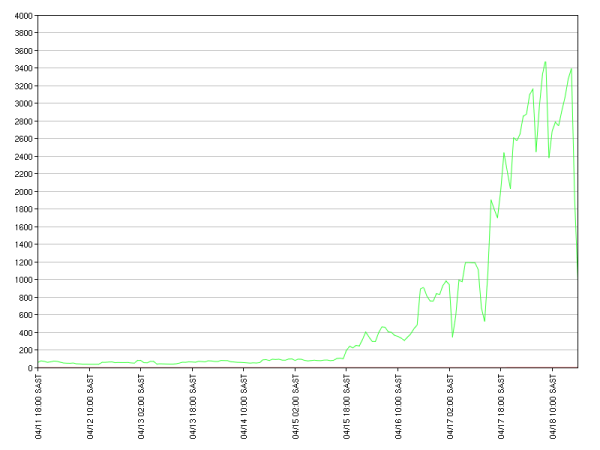
\includegraphics[width=.8\linewidth]{ec2-usage-animoto}
  \end{figure}
\end{frame}

\end{document}